\documentclass[a4paper]{article}
\usepackage{import}
\usepackage[utf8]{inputenc}
\usepackage[T1]{fontenc}
\usepackage{textcomp}
\usepackage[italian]{babel}
\usepackage{amsmath, amssymb}
\usepackage{booktabs,xltabular}
\usepackage{amsfonts}
\usepackage{subcaption}
\usepackage{amsthm}
\usepackage{cancel}
\usepackage{mdframed}
\usepackage{makecell}
\usepackage{float}
\usepackage{xcolor}
\usepackage{listings}
\usepackage{gensymb}
\usepackage{graphicx}
\usepackage{bodeplot}
\usepackage{physics}
\usepackage{tikz}
\usetikzlibrary{shapes, arrows, automata, petri, decorations.markings, decorations.pathreplacing, positioning, calc, quotes}
\usepackage{circuitikz}
\usepackage[label=corner]{karnaugh-map}
\graphicspath{{./figures/}}

% Set default font to sans-serif
\renewcommand{\familydefault}{\sfdefault} 
\usepackage{eulervm}

\usepackage{forest}

\usepackage{mathtools}
\DeclarePairedDelimiter\ceil{\lceil}{\rceil}
\DeclarePairedDelimiter\floor{\lfloor}{\rfloor}

% \usepackage{ntheorem}

\usepackage{import}
\usepackage{pdfpages}
\usepackage{transparent}
\usepackage{xcolor}

\usepackage{hyperref}
\hypersetup{
    colorlinks=false,
}

% Code blocks
\definecolor{codegreen}{rgb}{0,0.6,0}
\definecolor{codegray}{rgb}{0.5,0.5,0.5}
\definecolor{codepurple}{rgb}{0.58,0,0.82}
\definecolor{backcolour}{rgb}{0.95,0.95,0.95}

\lstdefinestyle{mystyle}{
	backgroundcolor=\color{backcolour},
	commentstyle=\color{codegreen},
	keywordstyle=\color{magenta},
	numberstyle=\tiny\color{codegray},
	stringstyle=\color{codepurple},
	basicstyle=\ttfamily\footnotesize,
	breakatwhitespace=false,
	breaklines=true,
	captionpos=b,
	keepspaces=true,
	numbers=left,
	numbersep=5pt,
	showspaces=false,
	showstringspaces=false,
	showtabs=false,
	tabsize=2
}

\lstset{style=mystyle}

\usepackage{color}
\usepackage{import}
\usepackage{pdfpages}
\usepackage{transparent}
\usepackage{xcolor}

% Example frame
\theoremstyle{definition}
\newmdtheoremenv[%
	linecolor=gray,leftmargin=0,%
	rightmargin=0,
	innertopmargin=8pt,%
	innerbottommargin=8pt,
	ntheorem]{example}{Esempio}[section]

% Important definition frame
\theoremstyle{definition}
\newmdtheoremenv[%
	linecolor=gray,leftmargin=0,%
	rightmargin=0,
	backgroundcolor=gray!40,%
	innertopmargin=8pt,%
	innerbottommargin=8pt,
	ntheorem]{definition}{Definizione}[section]

% Exercise frame
\theoremstyle{definition}
\newmdtheoremenv[%
	linecolor=gray,leftmargin=0,%
	rightmargin=0,
	innertopmargin=8pt,%
	innerbottommargin=8pt,
	ntheorem]{exercise}{Esercizio}[section]

% Theorem frame
\theoremstyle{definition}
\newmdtheoremenv[%
  linecolor=gray,leftmargin=0,%
  rightmargin=0,
  innertopmargin=8pt,%
  innerbottommargin=8pt,
  ntheorem]{theorem}{Teorema}[section]

\theoremstyle{definition}
\newmdtheoremenv[%
  linecolor=white,leftmargin=0,%
  rightmargin=0,
  innertopmargin=8pt,%
  innerbottommargin=8pt,
  ntheorem]{define}{Definizione utile}[section]

% figure support
\usepackage{import}
\usepackage{xifthen}
\pdfminorversion=7
\usepackage{pdfpages}
\usepackage{transparent}
\newcommand{\incfig}[1]{%
	\def\svgwidth{\columnwidth}
	\import{./figures/}{#1.pdf_tex}
}

% FSM tikz
\tikzset{
    place/.style={
        circle,
        thick,
        draw=black,
        minimum size=6mm,
    },
        state/.style={
        circle,
        thick,
        draw=black,
        fill=white,
        minimum size=6mm,
    },
}

\pdfsuppresswarningpagegroup=1

\usepackage{pgfplots}
\pgfplotsset{compat=1.18,width=10cm}

% Save plots as pdf and reuse them without compiling every time
\usetikzlibrary{external}
\tikzexternalize[prefix=figures/tikz/, optimize=false]


\begin{document}

\begin{titlepage}
	\begin{center}
		\vspace*{1cm}

		\Huge
		\textbf{Probabilità e Statistica\\Esercizi}

		\vspace{0.5cm}
		\LARGE
		UniVR - Dipartimento di Informatica

		\vspace{1.5cm}

		\textbf{Fabio Irimie}

		\vfill


		\vspace{0.8cm}


		2° Semestre 2023/2024

	\end{center}
\end{titlepage}


\tableofcontents
\pagebreak

\section{Introduzione}
Nel 1950 Alan Turing pubblica un articolo intitolato "Computing Machinery and Intelligence"
in cui propone un esperimento per determinare se una macchina può essere considerata
intelligente. L'esperimento, noto come "test di Turing", coinvolge un interrogatore umano
che comunica con due entità nascoste: una macchina e un essere umano. L'interrogatore deve
fare domande a entrambe le entità e, basandosi sulle risposte, deve determinare quale delle
due è la macchina. Se l'interrogatore non riesce a distinguere tra le risposte
della macchina e quelle dell'essere umano, la macchina è considerata intelligente.

\vspace{1em}
\noindent
In futuro l'attenzione si è spostata sulla ricerca di metodi per risolvere problemi che richiedono intelligenza
umana, utilizzando algoritmi e modelli matematici fino ad arrivare alle reti neurali e intelligenza artificiale.

\begin{definition}
  L'intelligenza artificiale è una disciplina che studia come \textbf{simulare} l'intelligenza umana in
  scenari complessi
\end{definition}

\subsection{Tipi di intelligenza artificiale}
\subsubsection{Autonomous agents}
Sono sistemi che percepiscono l'ambiente e agiscono in modo autonomo per raggiungere obiettivi specifici.

\subsubsection{Data analysis}
Utilizzo di algoritmi per analizzare grandi quantità di dati e estrarre informazioni utili e correlazioni
complesse.

\subsubsection{Machine Learning}
È lo sviluppo di algoritmi che permettono a dei modelli di apprendere dai dati
di esempio e migliorare le loro prestazioni nel tempo senza essere esplicitamente programmati.
Ad esempio riconoscimento di immagini.

L'apprendimento automatico è diviso in tre categorie principali:
\begin{itemize}
  \item \textbf{Unsupervised learning}: il modello viene addestrato su un insieme di dati non etichettati,
  dove l'obiettivo è scoprire strutture nascoste o pattern nei dati senza avere risposte corrette predefinite.
\item \textbf{Supervised learning}: il modello viene addestrato su un insieme di dati etichettati,
  dove ogni esempio di input è associato a una risposta corretta. L'obiettivo è che il modello impari a
  mappare gli input alle risposte corrette.
  \item \textbf{Reinforced learning}: il modello impara attraverso interazioni con l'ambiente, ricevendo
  ricompense o penalità in base alle azioni intraprese. L'obiettivo è massimizzare la ricompensa totale nel
  tempo.
\end{itemize}

\subsubsection{Time series analysis}
L'analisi delle serie temporali è un'area dell'apprendimento automatico che si concentra sull'analisi di dati
collezionati nel tempo. Le serie temporali sono sequenze di dati misurati a intervalli regolari, come
temperatura giornaliera, prezzi delle azioni o dati di vendita mensili. L'obiettivo dell'analisi delle
serie temporali è identificare pattern, tendenze e stagionalità nei dati per fare previsioni future.

\vspace{1em}
\noindent
Gli approcci comuni per l'analisi delle serie temporali includono:
\begin{itemize}
  \item \textbf{Riconoscimento di anomalie e cause}:
    è un processo di identificazione di dati o eventi che si discostano
    significativamente dal comportamento normale o atteso. Queste anomalie possono indicare problemi,
    errori o situazioni insolite che richiedono attenzione.

  \item \textbf{Generative transformers}:
    sono una classe di modelli che permettono di predirre il prossimo elemento in una
    sequenza di dati partendo dagli elementi precedenti, come ad esempio la parola successiva in una frase o il
    pixel successivo in un'immagine. Si sfrutta il concetto di \textbf{attenzione} per pesare l'importanza
    relativa delle diverse parti della sequenza di input durante la generazione dell'output.
\end{itemize}

\subsubsection{Intelligent Agents}
Un agente intelligente è un sistema che percepisce l'ambiente circostante attraverso sensori e agisce su
l'ambiente per raggiungere un obiettivo specifico. Gli elementi chiave di un agente intelligente includono:
\begin{itemize}
  \item \textbf{Performance measure}: misura il successo dell'agente nel raggiungere i suoi obiettivi
  \item \textbf{Rationality}: l'agente deve agire in modo da massimizzare la sua performance measure attesa
\end{itemize}

\subsection{Markov Decision Process (MDP)}
Un MDP è un modello matematico utilizzato per rappresentare problemi di decisione sequenziali. Gli elementi
principali sono:
\begin{itemize}
  \item \textbf{State}: rappresenta l'ambiente in un dato momento
  \item \textbf{Actions}: insieme delle azioni che l'agente può intraprendere
  \item \textbf{Transition model}: effetto che le azioni hanno sull'ambiente (potrebbero essere parzialmente incognite
    \[
      T: (state, action) \to next\_state
    \] 
  \item \textbf{Reward}: valore \textbf{immediato} dell'esecuzione di un'azione
    \[
      R: (state, action, next\_state) \to real\_number
    \] 
  \item \textbf{Policy}: strategia che l'agente utilizza per decidere quale azione intraprendere in ogni stato
    con l'obiettivo di massimizzare la ricompensa totale attesa nel tempo
    \[
      \pi: (state) \to action
    \] 
\end{itemize}

\subsection{Generative AI}
L'intelligenza artificiale generativa si riferisce a una classe di modelli di intelligenza artificiale
che sono in grado di generare nuovi contenuti, come testo, immagini, musica o video, a partire da dati di
addestramento. Questi modelli hanno miliardi di parametri e sono \textbf{preaddestrati} su grandi quantità
di dati. In sostanza questi modelli "predicono il futuro" basandosi sui dati su cui sono stati addestrati e
un \textbf{propmpt} (input dell'utente).

\section{Agenti e ambiente}
Gli agenti includono umani, robot, softbot, termostati ecc... La funzione dell'agente
mappa lo storico di percezioni in azioni:
\[
  f: \mathcal{P}^* \mapsto \mathcal{A}
\] 
Il programma dell'agente è eseguito su architettura fisica per produrre la funzione \( f \).
\begin{example}
  Un esempio potrebbe essere un insieme di stanze \( \{A, B\}  \) e un robot aspirapolvere che può
  percepire la sua posizione e il contenuto della stanza. L'agente potrebbe quindi percepire
  \( [A, Sporco] \) se ci fosse dello sporco nella stanza A. Le azioni potrebbero essere
  di movimento o pulizia. Tutto questo dipende dalla squenza di percezioni, ad esempio 
  in una tabella:
  \begin{table}[H]
    \centering
    \begin{tabular}{|c|c|}
      \hline
      Percezione & Azione \\
      \hline
      \( [A, Pulito] \) & Vai a B \\
      \( [A, Sporco] \) & Pulisci \\
      \( [B, Pulito] \) & Vai ad A \\
      \( [B, Sporco] \) & Pulisci \\
      \( [A, Pulito], [A, Pulito] \) & Vai a B \\
      \( [A, Pulito], [A, Sporco] \) & Pulisci \\
      \hline
    \end{tabular}
    \caption{Esempio di tabella di percezioni e azioni}
  \end{table}
  \noindent
  Non possiamo dire se questa è una funzione corretta perchè non abbiamo una
  \textbf{performance measure} che ci dica se l'agente sta facendo un buon lavoro.
\end{example}

\begin{definition}
  Se un agente ha \( \left| \mathcal{P} \right|  \) possibili percezioni, allora al tempo
  \( T \) avrà:
  \[
    \sum_{t=1}^{T} \left| \mathcal{P} \right|^t
  \] 
\end{definition}
\noindent
Se lo storico di percezioni è irrilevante, cioè se ad ogni percezione è associata un'azione
la funzione viene chiamata \textbf{Reflex}.

\subsection{Razionalità}
Per definire l'intelligenza di un agente si utilizza una misura di performance che
valuta la sequenza di percezioni.
\begin{example}
  Tornando all'esempio del robot aspirapolvere si potrebbero assegnare i seguenti
  punteggi:
  \begin{itemize}
    \item Un punto per ogni stanza pulita per ogni unità di tempo
    \item Meno un punto per ogni mossa
    \item Penalizzazione per ogni stanza sporca
  \end{itemize}
\end{example}

\begin{example}
  Un altro esempio è il seguente ambiente:
  \begin{itemize}
    \item Ci sono 3 stanze \( (A,B,C) \) e due robot \( (r_1, r_2) \) 
    \item \( r_1 \) può sorvegliare solo \( A \) e \( B \) e \( r_2 \) solo \( B \) e \( C \)
    \item \( r_1 \) inizia dalla stanza \( A \) e \( r_2 \) dalla \( C \)
    \item Il tempo di percorrenza tra le stanze è 0
    \item Performance measure: minimizza il tempo in cui una stanza non è sorvegliata,
      cioè il tempo totale in cui una stanza non è visitata da nessun robot
  \end{itemize}

  Un possibile comportamento razionale potrebbe essere il seguente (alternata):
  \begin{table}[H]
    \centering
    \begin{tabular}{|c|c|c||c|c|}
      \hline
      Stato & \( A \) & \( B \) & \( C \) & Tempo  \\
      \hline
      \( [A, C] \) & 0 & 1 & 0 & 1 \\
      \( [B, C] \) & 1 & 0 & 0 & 2 \\
      \( [A, C] \) & 0 & 1 & 0 & 3 \\
      \( [A, B] \) & 0 & 0 & 1 & 4 \\
      \hline
      Average idleness & \( \frac{1}{4} \)  & \( \frac{1}{2} \)  & \( \frac{1}{4} \)  & Tot: \( \frac{1}{3} \)  \\
      \hline
    \end{tabular}
  \end{table}
  \noindent
  Un altro comportamento potrebbe essere (fissata):
  \begin{table}[H]
    \centering
    \begin{tabular}{|c|c|c||c|c|}
      \hline
      Stato & \( A \) & \( B \) & \( C \) & Tempo  \\
      \hline
      \( [A, C] \) & 0 & 1 & 0 & 1 \\
      \( [B, C] \) & 1 & 0 & 0 & 2 \\
      \( [A, C] \) & 0 & 1 & 0 & 3 \\
      \( [B, C] \) & 1 & 0 & 0 & 4 \\
      \hline
      Average idleness & \( \frac{1}{2} \)  & \( \frac{1}{2} \)  & \( 0 \)  & Tot: \( \frac{1}{3} \)  \\
      \hline
    \end{tabular}
  \end{table}
  \noindent
  Entrambi i comportamenti hanno la stessa performance measure, ma il primo è migliore
  del secondo perchè penalizza meno una singola stanza rispetto alle altre. Per capirlo
  bisogna non solo minimizzare la performance measure, ma anche minimizzare la varianza.
\end{example}

\subsection{PEAS}
Per progettare un agente intelligente bisogna definire l'ambiente in cui opera:
\begin{itemize}
  \item \textbf{Performance measure}: come viene valutato il successo dell'agente
  \item \textbf{Environment}: il contesto in cui l'agente opera
  \item \textbf{Actuators}: i mezzi attraverso cui l'agente agisce sull'ambiente
  \item \textbf{Sensors}: i mezzi attraverso cui l'agente percepisce l'ambiente
\end{itemize}

\begin{example}
  Prendiamo ad esempio un taxi automatico, il PEAS potrebbe essere:
  \begin{itemize}
    \item Performance measure:
      \begin{itemize}
        \item Soddisfazione del cliente
        \item Sicurezza
        \item Efficienza del carburante
        \item Rispetto delle leggi stradali
      \end{itemize}
    \item Environment:
      \begin{itemize}
        \item Traffico stradale
        \item Condizioni meteorologiche
        \item Segnali stradali
        \item Pedoni e altri veicoli
      \end{itemize}
    \item Actuators:
      \begin{itemize}
        \item Volante
        \item Acceleratore
        \item Freni
        \item Indicatori di direzione
      \end{itemize}
    \item Sensors:
      \begin{itemize}
        \item Telecamere
        \item Lidar
        \item Radar
        \item Sensori di velocità
        \item GPS
      \end{itemize}
  \end{itemize}
\end{example}

\subsection{Tipi di ambienti}
Gli ambienti possono essere classificati in base a diverse caratteristiche:
\begin{itemize}
  \item \textbf{Osservabile}: se l'agente può percepire completamente lo stato dell'ambiente
    in ogni momento
  \item \textbf{Deterministico}: se l'azione dell'agente determina in modo univoco il prossimo stato
    dell'ambiente
  \item \textbf{Episodico}: se l'esperienza dell'agente è divisa in episodi indipendenti,
    cioè l'azione in un episodio non influisce sugli episodi successivi
  \item \textbf{Statico}: se l'ambiente non cambia mentre l'agente sta prendendo una
    decisione
  \item \textbf{Discreto}: se l'insieme di stati, azioni e percezioni è finito o numerabile
  \item \textbf{Singolo agente}: se l'agente opera da solo nell'ambiente senza la presenza
    di altri agenti
\end{itemize}
\begin{example}
  Prendiamo ad esempio i seguenti ambienti provando a classificarli:
  \begin{table}[H]
    \centering
    \begin{tabular}{|c|c|c|c|c|c|c|}
      \hline
      & Crossword & Robo-selector & Poker & Taxi \\
      \hline
      Osservabile & Sì & Parziale & Parziale & Parziale \\
      Deterministico & Sì & No & No & No \\
      Episodico & No & Sì & No & No \\
      Statico & Sì & No & Sì & No \\
      Discreto & Sì & No & Sì & No \\
      Singolo agente & Sì & Sì & No & No \\
      \hline
    \end{tabular}
  \end{table}
\end{example}
Il tipo di ambiente cambia radicalmente la soluzione del problema:
\begin{itemize}
  \item \textbf{Deterministico, completamente osservabile}: Single-state problem
  \item \textbf{Completamente non osservabile}: Conformant problem, l'agente non sa in che
    stato si trova, ma potrebbe trovare una soluzione
  \item \textbf{Non deterministico e/o parzialmente osservabile}: Contingency problem,
    l'agente deve prevedere le possibili situazioni future e agire di conseguenza
  \item \textbf{Spazio degli stati sconosciuto}: Exploration problem, l'agente deve esplorare
    l'ambiente per scoprire gli stati e le azioni disponibili
\end{itemize}

\subsection{Agenti di problem solving}
È una forma ristretta di agenti che formulato un problema e un obiettivo partendo da uno stato
cerca una soluzione ignorando le percezioni, siccome ci si trova in un single-state problem.
Questo si chiama Offline problem solving perchè l'agente ha completa conoscenza dell'ambiente.
Online problem solving è quando l'agente non ha completa conoscenza dell'ambiente.
\begin{example}
  Il seguente è un esempio di problem solving agent:
  \begin{lstlisting}[language=Python]
function Simple-Problem-Solving-Agent(percept) returns action
  static: seq, an action sequence, initially empty
          state, some description of the current world state
          goal, a goal, initially null
          problem, a problem formulation

  state <- Update-State(state, percept)

  if seq is empty then
    goal <- Formulate-Goal(state)
    problem <- Formulate-Problem(state, goal)
    seq <- Search( problem)

  action <- First(seq)
  seq <- Rest(seq)
  return action
  \end{lstlisting}
\end{example}
\begin{example}
  Consideriamo il problema "Vacanze in Romania". Bisogna formulare un viaggio da Arad a
  Bucarest sapendo che l'aereo parte domani.
  \begin{itemize}
    \item \textbf{Goal}: Arrivare a Bucarest
    \item \textbf{Formulazione del problema}:
      \begin{itemize}
        \item Stati: città della Romania
        \item Azioni: volare tra le città
      \end{itemize}
    \item \textbf{Soluzione}: Sequenza di città
  \end{itemize}
  \noindent
  Si potrebbe usare una mappa per trovare il percorso più breve (visione completa del mondo)
  e trovare una soluzione ottimale.
  Questo problema è definito da 4 componenti:
  \begin{itemize}
    \item \textbf{Stato iniziale}: ad esempio "ad Arad"
    \item \textbf{Funzione di transizione}: insieme di coppie (stato, azione) che mappano
      uno stato in un altro, ad esempio:
      \[
        S(A) = \left\{ \left< \text{Arad} \to \text{Zerind}, \text{Zerind} \right>, \ldots \right\}
      \] 
    \item \textbf{Test dell'obiettivo}: una funzione che verifica se lo stato corrente
      soddisfa l'obiettivo, ad esempio:
      \[
        Goal\text{-}Test(s) = \begin{cases}
          \text{true} & \text{se } s = \text{Bucarest} \\
          \text{false} & \text{altrimenti}
        \end{cases}
      \]
    \item \textbf{Path cost}: è una funzione che assegna un costo (additivo) a ogni azione,
      ad esempio la somma di distanze o il numero di azioni:
      \[
        c(x, a, y) \ge 0
      \] 
    \item \textbf{Soluzione}: Una sequenza di azioni che portano dallo stato iniziale allo
      stato obiettivo.
  \end{itemize}
\end{example}

\section{Ricerca nello spazio degli stati}
\subsection{Ricerca generale}
\subsubsection{Tree search}
Un algoritmo di ricerca ad albero esplora lo spazio degli stati partendo dallo stato iniziale
e generando nuovi stati (successori) applicando le azioni disponibili, cioè 
\textbf{espandendo} gli stati:
\begin{lstlisting}[language=Python]
function Tree-Search(problem, strategy) runction Tree-Search( problem, strategy) returns a solution, or failure
initialize the search tree using the initial state of problem
loop do
if no candidates for expansion then return failure
choose a leaf node for expansion according to strategy
if node contains a goal state then return the solution
else add successor nodes to the search tree (expansion)
endeturns a solution, or failure
  initialize the search tree using the initial state of problem
  loop do
    if no candidates for expansion then return failure
      choose a leaf node for expansion according to strategy
    if node contains a goal state then return the solution
      else add successor nodes to the search tree (expansion)
end
\end{lstlisting}

\subsubsection{Stato e nodo}
Stato e nodo non sono la stessa cosa, infatti:
\begin{itemize}
  \item \textbf{Stato}: rappresenta una configurazione dell'ambiente
  \item \textbf{Nodo}: è una struttura dati che costituisce una parte dell'albero di ricerca
    e include informazioni aggiuntive come il genitore, l'azione che ha portato a quello stato,
    il costo del percorso o la profondità nell'albero, ecc...
\end{itemize}

\subsubsection{Tree search generale}
Espandere un nodo significa generare i suoi figli, cioè i nodi successori e tutti i nodi
non esplorati sono chiamati \textbf{frontiera}.
\begin{lstlisting}[language=Python]
function Tree-Search( problem, frontier) returns a solution, or failure
  frontier <- Insert(Make-Node(problem.Initial-State))
  while not IsEmty(frontier) do
    node <- Pop(frontier)
    if problem.Goal-Test(node.State) then return node
      frontier <- InsertAll(Expand(node, problem))
  end loop
  return failure
\end{lstlisting}
La strategia è quella di scegliere l'ordine in cui i nodi vengono espansi, cioè
come viene gestita la frontiera. Le strategie sono valutate in base a:
\begin{itemize}
  \item \textbf{Completezza}: se garantisce di trovare una soluzione quando esiste
  \item \textbf{Complessità di tempo}: numero di nodi generati o espansi
  \item \textbf{Complessità di spazio}: numero massimo di nodi memorizzati in memoria
  \item \textbf{Ottimalità}: se garantisce di trovare la soluzione migliore
\end{itemize}
Le complessità di spazio e di tempo sono misurate in termini di:
\begin{itemize}
  \item \( b \): maximum branching factor, numero massimo di figli per nodo
  \item \( d \): profondità della soluzione meno costosa
  \item \( m \): profondità massima dell'albero di ricerca (potrebbe essere infinita)
\end{itemize}

\subsubsection{Stati ripetuti}
Fallire nel riconoscere stati ripetuti può trasformare un problema lineare in un problema
esponenziale. Bisogna quindi mantenere una lista di stati già visitati e non espandere
nodi che portano a stati già visitati:
\begin{lstlisting}[language=Python]
function Graph-Search( problem, frontier) returns a solution, or failure
  explored <- an empty set
  frontier <- Insert(Make-Node(problem.Initial-State))
  while not IsEmty(frontier) do
    node <- Pop(frontier)
    if problem.Goal-Test(node.State) then return node
    if node.State is not in explored then
      add node.State to explored
      frontier <- InsertAll(Expand(node, problem))
    end if
  end loop
  return failure
\end{lstlisting}

\subsection{Ricerca non informata}
Gli algoritmi di ricerca non informata utilizzano soltanto i dati disponibili nella
definizione del problema e i principali sono:
\begin{itemize}
  \item Breadth-first search
  \item Uniform-cost search (Dijkstra)
  \item Depth-first search
  \item Depth-limited search
  \item Iterative deepening search
\end{itemize}

\subsubsection{Breadth-first search}
Questo algoritmo espande il nodo non esplorato più superficiale, cioè il nodo più vicino
alla radice. Utilizza una coda FIFO per la frontiera e i nuovi successori vengono
aggiunti alla fine della coda.
\begin{lstlisting}[language=Python]
function BFS( problem) returns a solution, or failure
  node <- node with State=problem.Initial-State,Path-Cost=0
  if problem.Goal-Test(node.State) then return node
  explored <- empty set frontier <- FIFO queue with node as the only element
  loop do
    if frontier is empty then return failure
    node <- Pop(frontier)
    add node.State to explored
    for each action in problem.Actions(node.State) do
      child <- Child-Node(problem,node,action)
      if child.State is not in (explored or frontier) then
        if problem.Goal-Test(child.State) then return child
        frontier <- Insert(child)
      end if
    end for
  end loop
\end{lstlisting}
\noindent
Questo tipo di ricerca è:
\begin{itemize}
  \item \textbf{Completa}: Sì, soltanto se \( b \) è finito, cioè se il branching factor
    è limitato
  \item \textbf{Complessità di tempo}: \( b + b^2 + b^3 + \ldots + b^d = O(b^d) \)
  \item \textbf{Complessità di spazio}: \( O(b^d) \), perchè bisogna memorizzare tutti i nodi
    generati
  \item \textbf{Ottimale}: Sì, soltanto se il costo delle azioni è uniforme
\end{itemize}

\subsubsection{Uniform-cost search}
Questo algoritmo espande il nodo non esplorato con il \textbf{costo del percorso più basso}.
La frontiera è una coda di priorità ordinata in base al costo del percorso.
Questo tipo di ricerca è:
\begin{itemize}
  \item \textbf{Completa}: Sì, se il costo minimo delle azioni \( \ge \varepsilon \) 
    (con piccola ma \( \varepsilon > 0 \))
  \item \textbf{Complessità di tempo}: Numero di nodi \( g \le  \) del costo del percorso
    ottimale \( C^* \). \( O(b^{1+\lfloor C^*/\epsilon \rfloor}) \)
  \item \textbf{Complessità di spazio}: \( O(b^{1+\lfloor C^*/\epsilon \rfloor}) \)
  \item \textbf{Ottimale}: Sì perchè i nodi vengono espansi in ordine di costo del percorso
\end{itemize}
Ci sono due modifiche principali rispetto alla BFS che garantiscono l'ottimalità:
\begin{enumerate}
  \item Il goal test viene fatto quando il nodo viene estratto dalla frontiera, non quando
    viene generato. (Questo elemento spiega il \( +1 \) nella complessità
  \item Controllare se un nodo generato è già presente nella frontiera con un costo più
    alto e in tal caso sostituirlo con il nuovo nodo a costo più basso
\end{enumerate}

\subsubsection{Depth-first search}
Questo algoritmo espande il nodo non esplorato più profondo, cioè il nodo più lontano
dalla radice. Utilizza una pila LIFO per la frontiera e i nuovi successori vengono
aggiunti all'inizio.
Questo tipo di ricerca è:
\begin{itemize}
  \item \textbf{Completa}: No, perchè può rimanere bloccata in un ramo infinito,
    a meno che l'albero di ricerca non abbia una profondità limitata. Si potrebbero
    evitare loop modificando l'algoritmo per evitare stati ripetuti sul percorso corrente
  \item \textbf{Complessità di tempo}: \( O(b^m) \), dove \( m \) è la profondità massima
    dell'albero di ricerca
  \item \textbf{Complessità di spazio}: \( O(bm) \), bisogna memorizzare soltanto il
    percorso corrente e i nodi fratelli
  \item \textbf{Ottimale}: No, perchè non garantisce di trovare la soluzione migliore
\end{itemize}

\subsubsection{Iterative deepening search}
Questo algoritmo combina i vantaggi della BFS e della DFS. Esegue una serie di ricerche
in profondità limitata, aumentando progressivamente il limite di profondità fino a
trovare una soluzione.
\begin{lstlisting}[language=Python]
# Depth-Limited Search
function DLS(problem, limit) returns soln/fail/cutoff
  R-DLS(Make-Node(problem.Initial-State), problem, limit)


function R-DLS(node, problem, limit) returns soln/fail/cutoff
  if problem.Goal-Test(node.State) then return node
  else if limit = 0 then return cutoff # raggiunta la profondita' massima
  else
    # flag: c'e' stato un cutoff in uno dei sottoalberi?
    cutoff-occurred? <- false
    for each action in problem.Actions(node.State) do
      child <- Child-Node(problem, node, action)
      result <- R-DLS(child, problem, limit-1)
      if result = cutoff then cutoff-occurred? <- true
      else if result 6 = failure then return result
    end for
    if cutoff-occurred? then return cutoff else return failure
  end else

# Iterative Deepening Search
function IDS(problem) returns a solution
  inputs: problem, a problem
  for depth <- 0 to infinity do
    result <- DLS(problem, depth)
    if result 6 = cutoff then return result
  end
\end{lstlisting}
Questo tipo di ricerca è:
\begin{itemize}
  \item \textbf{Completa}: Sì
  \item \textbf{Complessità di tempo}: \( db^1 + (d-1)b^2 + \ldots + b^d = O(b^d) \) 
  \item \textbf{Complessità di spazio}: \( O(bd) \) 
  \item \textbf{Ottimale}: Sì, se il costo delle azioni è uniforme
\end{itemize}

\begin{exercise}
  Assumi:
  \begin{enumerate}
    \item Un albero di ricerca ben bilanciato, tutti i nodi hanno lo stesso numero di figli
    \item Il goal state è l'ultimo che viene espanso nel suo livello (il più a destra)
    \item Se il branching factor è 3, la soluzione più superficiale è a profondità 3
      (la radice è a profondità 0) e si utilizza la ricerca in ampiezza quanti nodi
      vengono generati?
    \item Se il branching factor è 3, la soluzione più superficiale è a profondità 3
      (la radice è a profondità 0) e si utilizza la iterative deepening quanti nodi
      vengono generati?
  \end{enumerate}
\end{exercise}
\begin{exercise}
  Un uomo ha un lupo, una pecora e un cavolo. L'uomo è sulla riva di un fiume con una
  barca che può trasportare solo lui e un altro oggetto. Il lupo mangia la pecora e la
  pecora mangia il cavolo, quindi non può lasciarli insieme da soli.
  \begin{enumerate}
    \item Formalizza il problema come un problema di ricerca
    \item Usa BFS per risolvere il problema
  \end{enumerate}

  \vspace{1em}
  \noindent
  \textbf{Soluzione:}

  Formalizziamo gli stati come una tupla:
  \[
    <W, S, C, M, B>
  \] 
  dove:
  \begin{itemize}
    \item \( W \): posizione del lupo
    \item \( S \): posizione della pecora
    \item \( C \): posizione del cavolo
    \item \( M \): posizione dell'uomo
    \item \( B \): stato della barca
  \end{itemize}
  La posizione può essere \( 0 \) (left) o \( 1 \) (right).

  Lo stato iniziale è:
  \[
    <0, 0, 0, 0, 0>
  \] 
  Lo stato obiettivo è:
  \[
    <1, 1, 1, 1, 1>
  \]
  Le azioni possibili sono:
  \begin{itemize}
    \item Porta il lupo (CW)
    \item Porta la pecora (CS)
    \item Porta il cavolo (CC)
    \item Porta niente (CN)
  \end{itemize}
  \begin{table}[H]
    \centering
    \begin{tabular}{|c|c|c|}
      \hline
      Operatore & Precondizione & Funzione \\
      \hline
      \footnotesize CW & \footnotesize \( M = B, M = W, S \neq C \) & \footnotesize\( \left<W,S,C,M,B\right> \mapsto \left<\bar{W},S,C,\bar{M},\bar{B}\right> \)\\
      \footnotesize CS & \footnotesize \( M = B, M = S \) & \footnotesize\( \left<W,S,C,M,B\right> \mapsto \left<W,\bar{S},C,\bar{M},\bar{B}\right> \)\\
      \footnotesize CC & \footnotesize \( M = B, M = C, W \neq S \) & \footnotesize\( \left<W,S,C,M,B\right> \mapsto \left<W,S,\bar{C},\bar{M},\bar{B}\right> \)\\
      \footnotesize CN & \footnotesize \( M = B \) & \footnotesize\( \left<W,S,C,M,B\right> \mapsto \left<W,S,C,\bar{M},\bar{B}\right> \)\\
      \hline
    \end{tabular}
  \end{table}
  Notiamo che in tutte le precondizioni c'è \( M = B \) perchè l'uomo deve essere
  sempre con la barca, quindi si possono unire i due stati in uno solo \( M \).
\end{exercise}

\subsection{Ricerca informata}
Gli algoritmi di ricerca informata utilizzano informazioni aggiuntive (euristiche)
per guidare la ricerca verso la soluzione in modo più efficiente.

\subsubsection{Best-first search}
Questo algoritmo usa una \textbf{funzione di valutazione} per ogni nodo che stima la
"desiderabilità". La frontiera è una coda ordinata in ordine decrescente di desiderabilità.
A seconda di come viene definita la desiderabilità si ottengono diversi algoritmi:
\begin{itemize}
  \item Greedy best-first search
  \item A*
\end{itemize}

\subsubsection{Greedy best-first search}
Questo algoritmo espande il nodo che sembra essere il più vicino alla soluzione
secondo una funzione di valutazione euristica \( h(n) \) che stima il costo
rimanente per raggiungere l'obiettivo da un nodo \( n \).
\begin{example}
  In una mappa di una città, la funzione di valutazione potrebbe essere la distanza
  in linea d'aria dal nodo corrente alla destinazione. In questo modo, l'algoritmo
  esplora prima i nodi che sembrano più vicini alla destinazione, riducendo il numero
  di nodi esplorati rispetto a una ricerca non informata.
\end{example}
Questo tipo di ricerca è:
\begin{itemize}
  \item \textbf{Completa}: No, perchè può rimanere bloccata in un ciclo infinito. È
    completo se lo spazio di ricerca è finito e ci sono controlli per evitare stati
    ripetuti
  \item \textbf{Complessità di tempo}: \( O(b^m) \) nel peggiore dei casi, ma può essere
    molto più veloce con una buona euristica
  \item \textbf{Complessità di spazio}: \( O(b^m) \), bisogna memorizzare tutti i nodi
    generati
  \item \textbf{Ottimale}: No
\end{itemize}

\subsubsection{A* search}
Questo algoritmo evita di espandere cammini che sono già molto costosi e ha come
funzione di valutazione:
\[
  f(n) = g(n) + h(n)
\] 
dove:
\begin{itemize}
  \item \( g(n) \): costo del percorso dal nodo iniziale a \( n \)
  \item \( h(n) \): stima del costo rimanente per raggiungere l'obiettivo da \( n \)
  \item \( f(n) \): stima del costo totale del percorso passando per \( n \)
\end{itemize}
L'euristica, per poter garantire l'ottimalità, deve essere \textbf{ammissibile}, cioè
per ogni nodo la stima di quel nodo deve essere minore o uguale del vero costo per arrivare
all'obbiettivo, quindi non deve \textbf{sovrastimare} il costo rimanente:
\[
  h(n) \le h^*(n) \quad h(n) \ge 0 \to h(G) = 0
\] 
dove \( h^*(n) \) è il costo effettivo del percorso da \( n \).
\begin{theorem}
  Per A* l'euristica ammissibile implica l'ottimalità
\end{theorem}
\noindent
Questo tipo di ricerca è:
\begin{itemize}
  \item \textbf{Completa}: Sì, tranne se ci sono infiniti nodi con \( f \le f(G) \) 
  \item \textbf{Complessità di tempo}: Esponenziale in errore relativo in \( h \times  \) 
    lunghezza del numeo di passi della soluzione ottimale. (Se l'euristica è buona, la
    complessità sarà molto più bassa)
  \item \textbf{Complessità di spazio}: \( O(b^d) \), bisogna memorizzare tutti i nodi
    generati
  \item \textbf{Ottimale}: Sì, ma richiede assunzioni sull'euristica (ammissibilità,
    consistenza) e una strategia di ricerca (ricerca ad albero o grafo)
\end{itemize}

\subsubsection{Consistenza e ammissibilità}
\begin{definition}
  Un euristica è \textbf{consistente} se:
  \[
    h(n) \le c(n,a,n') + h(n')
  \] 
  \begin{figure}[H]
    \centering
    \begin{tikzpicture}[->, node distance=2cm, on grid, auto]
      \node[state] (n) {$n$};

      \node[state, below of=n] (n1) {$n'$};

      \node[state, below right of=n1] (G) {$G$};

      \draw (n) edge[left] node{\( c(n,a,n') \)} (n1);
      \draw (n) edge[right] node{\( h(n) \)} (G);
      \draw (n1) edge[left] node{\( h(n') \)} (G);
    \end{tikzpicture}
    \caption{Esempio di euristica consistente}
  \end{figure}
  \begin{itemize}
    \item Si può dimostrare che se \( h \) è consistente, allora \( f(n) \) non decresce
      lungo qualsiasi cammino

    \item A* espande i nodi in ordine crescente di \( f \), quindi trova sempre la soluzione
      ottimale
  \end{itemize}
  Quindi si espande sempre prima un cammino ottimo rispetto a un cammino non ottimo.
\end{definition}

\noindent
La consistenza implica l'ammissibilità e può essere dimostrato per induzione sul cammino
verso il goal. L'ammissibilità però non implica la consistenza.
\[
  \begin{aligned}
    \text{Consistenza} \to \text{Ammissibilità}\\
    \text{Ammissibilità} \not\to \text{Consistenza}
  \end{aligned}
\] 
\begin{itemize}
  \item Tree-Search + euristica ammissibile \( \to \) A* ottimale
  \item Graph-Search + euristica ammissibile \( \not\to \) A* ottimale (può scartare
    il cammino ottimale per un nodo ripetuto)
  \item Graph-Search + euristica consistente \( \to \) A* ottimale
\end{itemize}

\subsubsection{Euristiche}
Le euristiche possono essere create in diversi modi, prendiamo ad esempio l'8-puzzle:
\begin{figure}[H]
  \centering
  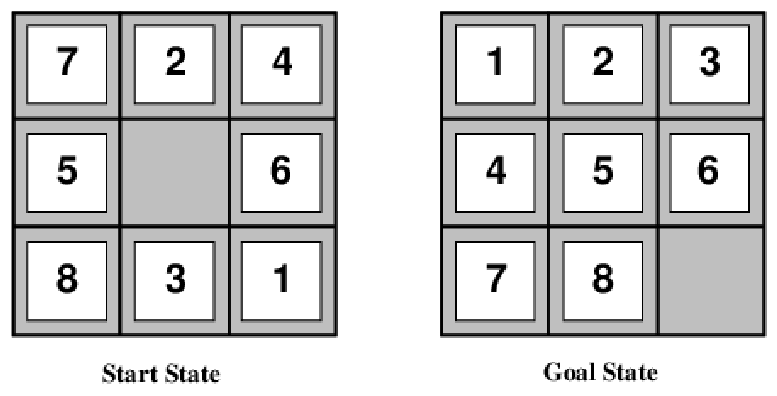
\includegraphics[width=0.8\textwidth]{8-puzzle}
  \caption{Esempio di 8-puzzle}
\end{figure}
Per questo problema si potrebbe utilizzare come euristica:
\begin{itemize}
  \item \( h_1(n) = \) numero di pezzi fuori posto
  \item \( h_2(n) = \) somma delle distanze di Manhattan (numero di mosse orizzontali e verticali
    necessarie per portare ogni pezzo alla sua posizione obiettivo)
\end{itemize}
Entrambe le euristiche sono ammissibili, ma \( h_2 \) è più precisa di \( h_1 \) perchè
fornisce una stima più vicina al costo reale per raggiungere l'obiettivo.

In questo caso si dice che \( h_2 \) \textbf{domina} \( h_1 \) se sono entrambe ammissibili
e \( h_2(n) \) è sempre maggiore o uguale a \( h_1 \):
\[
  h_2(n) \ge h_1(n) \quad \forall n
\] 

\begin{theorem}
  Date due qualsiasi euristiche \textbf{ammissibili} \( h_a \) e \( h_b \),
  allora l'euristica definita come:
  \[
    h(n) = \max(h_a(n), h_b(n))
  \]
  è anch'essa ammissibile e domina sia \( h_a \) che \( h_b \)
\end{theorem}

\noindent
Le euristiche ammissiibli possono essere derivate dall'esatto costo della soluzione di un
problema \textbf{rilassato}, cioè un problema simile a quello originale ma con
restrizioni rimosse. Ad esempio, per l'8-puzzle si potrebbe rilassare il problema
permettendo di muovere una casella ovunque (in questo caso \( h_1(n) \) da la soluzione
migliore), oppure permettendo di muovere una casella in qualsiasi casella adiacente (
in questo caso \( h_2(n) \) da la soluzione migliore)

\begin{define}
  Il costo della soluzione ottimale di un problema rilassato non è maggiore del costo
  della soluzione ottimale del problema reale.
\end{define}

\end{document}
